\documentclass[tikz,convert={outext=.svg,command=\unexpanded{{pdf2svg \infile\space \outfile}}}]{standalone}

\usetikzlibrary{automata,positioning,arrows.meta}

\tikzset{
%-{Stealth[length=3mm,width=2mm]}, % makes the edges directed
>={Stealth[length=3mm,width=2mm]}, % makes the arrow heads bold
node distance=3cm, % specifies the minimum distance between two nodes. Change if necessary.
every state/.style={ultra thick},
every path/.style={color=white,thick},
every node/.style={font=\Large,align=center},
initial text=$ $,
on grid,
auto
}


\begin{document}

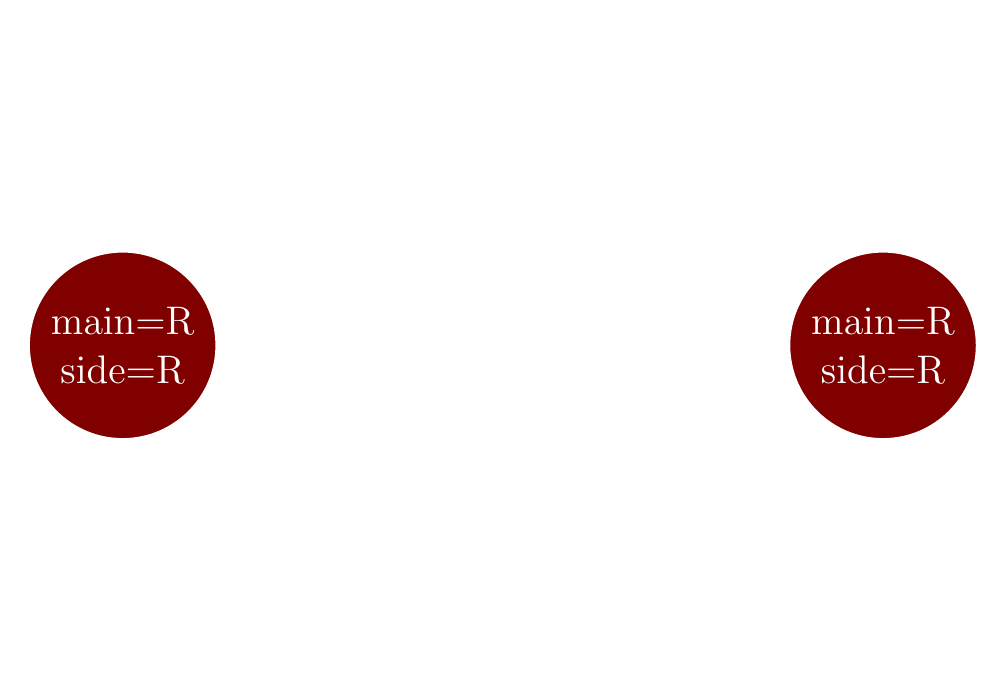
\begin{tikzpicture}[state/.style={circle, draw, minimum size=1.5cm, node distance=4cm}]
   \node[state] (rr1) [fill=red!50!black] {main=R \\ side=R};
   \node[state] (rg)  [above right=of rr1] {main=R \\ side=G};
   \node[state] (ry)  [right=of rg] {main=R \\ side=Y};
   \node[state] (rr2) [below right=of ry, fill=red!50!black] {main=R \\ side=R};
   \node[state] (gr)  [below left=of rr2] {main=G \\ side=R};
   \node[state] (yr)  [left=of gr] {main=Y \\ side=R};
   \path[->]
    (rr1) edge (rg)
    (rg)  edge (ry)
    (ry)  edge (rr2)
    (rr2) edge (gr)
    (gr)  edge (yr)
    (yr)  edge (rr1);
\end{tikzpicture}
\end{document}
